\documentclass[10pt, a4paper]{article}
\usepackage{ctex}
\usepackage{amsfonts}
\usepackage{amsmath}
\usepackage{amssymb, bm}
\usepackage{algorithm}
\usepackage{algpseudocode}
\usepackage{hyperref}
\usepackage[top=25.4mm, bottom=25.4mm, left=31.7mm, right=32.2mm]{geometry}
\usepackage{graphicx}
\usepackage{subfigure}


\setmainfont{Times New Roman}
\newtheorem{property}{性质}[section]
\newtheorem{thm}{定理}[section]
\newtheorem{definition}{定义}[section]
\renewcommand{\algorithmicrequire}{\textbf{输入:}}
\renewcommand{\algorithmicensure}{\textbf{输出:}}

\usepackage[
    style=numeric,
    sorting=none,
    bibstyle=gb7714-2015,
    citestyle=gb7714-2015
]{biblatex}

\renewcommand{\bibfont}{\zihao{-5}}

\addbibresource{reference.bib}

\begin{document}
\begin{titlepage}
\pagenumbering{Roman}
\author{张皓飞 (11921056)}
\title{语义分割模型:DeepLab}
\maketitle
\thispagestyle{empty}
\end{titlepage}

\newpage
\tableofcontents
\newpage
\pagenumbering{arabic}

\section{引言}
\subsection{计算机视觉中的任务}
计算机视觉想要解决的问题就是如何让机器真正理解一张输入图片,那么首先,机器必须要知道这张图片所描述的对象是什么。
比较简单的做法就是将所有图像描述的对象划分成一系列的类别,并对输入的图片根据划分好的类别进行分类,这样机器就可以
获得输入图片的最基本语义信息。因此分类问题就是计算机视觉中是一个至关重要的任务。

传统的解决分类的任务为先根据输入的图片的大致分布人为构建一系列特征提取器,比较有名的特征提取器为SIFT\cite{SIFT}、
SURF\cite{SURF}和HOG\cite{HOG}等。这些特征提取器将输入的图像变换为具有固定长度的向量,之后再使用线性分类器如
Rosenblatt感知机\cite{Rosenblatt}、贝叶斯分类器\cite{SimonNNLM}和支持向量机(SVM)\cite{SVM-Kernel}等
或非线性的分类器如决策树\cite{DataMining}、基于核方法的支持向量机\cite{SVM-Kernel}进行分类。

尽管这些传统的图像分类算法具有严格证明的数学定理和证明做支撑,但由于分类器以及研究得非常透彻,以至于大部分的算法
构建时间都会用在如何从图像提取特征的问题,也称为“特征工程”。由于图像的分布对于不同的任务差异巨大,以至于这些
特征工程算法很难进行泛化和推广,因此研究人员需要花费大量的时间进行模型的调参,从而得到令人满意的结果。

随着计算机软硬件和互联网的蓬勃发展,研究人员可以获得大量的数据,然而模型的效果并没有随着数据量的增加而显著提高,
而于此同时,基于卷积神经网络的分类器却显著地由于传统的特征工程方法。在2012年的ILSVRC\cite{ILSVRC}的比赛中
Alex Krizhevsky通过训练卷积神经网络AlexNet\cite{AlexNet}并获得了冠军。

尽管卷积神经网络并没有像传统机器学习一样具有很强的可解释性,但由于其可表述更强的非线性性和更大的参数空间,使得
深度模型可以往往收敛到较传统方法更优的模型。

\subsection{语义分割任务}
有了对图片的分类,机器可以初步理解图像所表示的类别,但是通常图片里具有多个物体,每个物体可能都属于不同的类别,
因此我们希望机器可以对一张图片的所有物体全部标记在图像中,从而可以获取到图片中更多的信息。从本质上将,
语义分割任务即对输入的图片的每个像素点进行分类,并将相同类别的像素点进行组合,从而得到物体对应的位置。

有了对图片的语义分割,我们可以获得更高层次的语义信息。在自动驾驶、人机交互和虚拟现实等诸多应用中都需要输入图片的
更高层次的语义信息。因此语义分割任务也是计算机视觉里重要的任务之一。

本文中将介绍一种基于深度卷积网络的语义分割模型DeepLab\cite{Deeplab1,Deeplab2,Deeplab3}系列,
该算法在Pascal VOC数据集\cite{VOC}和MSCOCO数据集\cite{COCO}取得了当时较好的结果。

\section{相关工作}
\subsection{语义分割任务}
关于深度卷积网络(DCNNs)在像素级语义分割中有大致三种主要方法:

\begin{description}
    \item[基于区域的语义分割] 基于区域的方法通常基于目标检测架构如R-CNN\cite{RCNN}等,对于分割的任务,R-CNN首先利用
    选择性搜索提取大量的候选区域,并计算其对应的特征。之后再使用线性分类模型对每个区域进行分类,再将区域的预测转换为
    像素预测。这种方法通常无法端到端实现,计算量较大。
    \item[弱监督语义分割] 通常对语义分割的数据集的标注是非常繁琐的,为此许多方法提出使用边框注释来作为监督信息训练
    模型,而非像素级的标注如BoxSup\cite{BoxSup}算法致力于通过使用带注释的边界框来实现语义分割。
    \item[全卷积网络语义分割] 全卷积网络可以对输入的图像进行端到端的语义分割,从而使得语义分割模型可以快速且方便的训练。
    全卷积网络大致可看成为编码器-解码器架构,其中编码器部分从图像中提取特征,解码器部分将提取到的特征恢复为语义分割的图像,
    如图\ref{p1}所示。目前,FCNs\cite{FCN}、SegNet\cite{SegNet}、U-Net\cite{UNet}以及DeepLab系列模型都为基于全卷积的
    语义分割模型。

    \begin{figure}
        \label{p1}
        \centering
        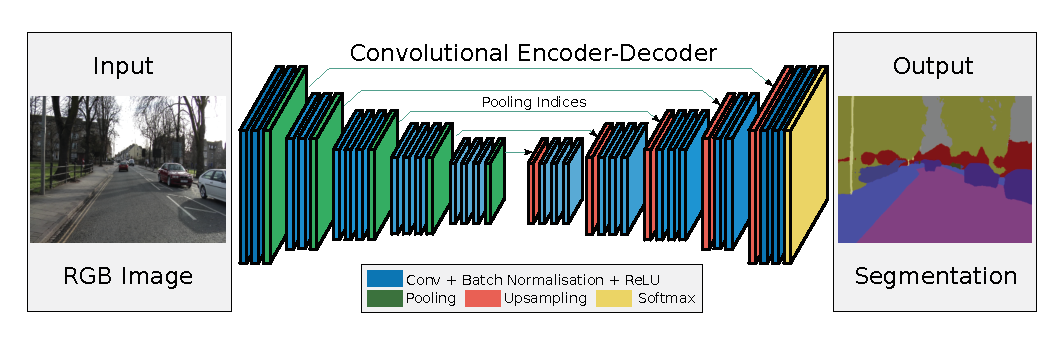
\includegraphics[width=\textwidth]{p1.eps}
        \caption{编解码器示例\cite{SegNet}}
    \end{figure}
\end{description}

\section{方法}
\subsection{DeepLab-V1}



\subsection{DeepLab-V2}

\section{实验结果}

\section{总结}


\newpage
\addcontentsline{toc}{section}{参考文献}
\nocite{*}
\printbibliography[heading=bibliography,title=参考文献]

\end{document}
